\chapter{Introdução}

A computação gráfica é a área da ciência da computação que estuda a geração, manipulação e exibição de imagens digitais. O que começou como uma forma simples de desenhar linhas em telas de osciloscópios evoluiu para uma disciplina fundamental que sustenta indústrias multibilionárias. Este volume foca nos alicerces técnicos que permitem transformar dados matemáticos abstratos em experiências visuais ricas. A compreensão profunda desses conceitos permite que desenvolvedores e artistas criem simulações que desafiam a percepção da realidade, unindo matemática, física e percepção humana em um único campo de estudo.

\section{Uma Breve História}

A jornada da computação gráfica moderna começou em 1963 com Ivan Sutherland e seu sistema \textit{Sketchpad}. Este projeto foi revolucionário ao introduzir o uso de uma caneta ótica para manipular objetos geométricos diretamente na tela, estabelecendo os conceitos de interface gráfica e hierarquia de objetos. Sutherland demonstrou que computadores poderiam ser usados para muito mais do que apenas cálculos numéricos puros, abrindo as portas para o design assistido por computador (CAD) e para a manipulação visual interativa.

Nas décadas de 1970 e 1980, a área viu um crescimento explosivo. A fundação do SIGGRAPH (\textit{Special Interest Group on Computer Graphics and Interactive Techniques}) em 1974 criou o fórum principal para a publicação de algoritmos que usamos até hoje. Em 1975, \textcite{phong1975illumination} introduziu um modelo de iluminação que permitiu superfícies mais realistas com brilhos especulares, resolvendo problemas de descontinuidade visual em malhas poligonais. Pouco depois, em 1980, Turner Whitted publicou as bases do \textit{Ray Tracing} recursivo, permitindo reflexões e refrações fidedignas, o que marcou o início da busca pelo fotorrealismo global.

No cinema, a evolução foi marcada por marcos como \textit{Tron} (1982), que usou CGI de forma extensiva, e \textit{Toy Story} (1995), o primeiro longa-metragem totalmente gerado por computador. Recentemente, a revolução do tempo real, impulsionada pelo desenvolvimento de GPUs (\textit{Graphics Processing Units}) cada vez mais poderosas, trouxe gráficos de qualidade cinematográfica para os jogos eletrônicos e simulações interativas. A introdução de técnicas de \textit{Real-Time Ray Tracing} e o uso de inteligência artificial para reconstrução de imagem (como o DLSS e FSR) representam o estado da arte atual.

\section{Aplicações Modernas}

Atualmente, os conceitos que estudaremos neste livro são aplicados em diversas frentes:

\begin{itemize}
    \item \textbf{Jogos Eletrônicos:} Renderização de ambientes complexos a 60 quadros por segundo ou mais, exigindo otimização extrema e uso eficiente do hardware.
    \item \textbf{Cinema e Efeitos Visuais:} Criação de mundos e criaturas que se misturam perfeitamente com filmagens reais, muitas vezes utilizando técnicas de renderização offline que levam horas para processar um único quadro.
    \item \textbf{Visualização Científica e Médica:} Representação de dados complexos, como tomografias computadorizadas e simulações de dinâmica de fluidos, permitindo que pesquisadores identifiquem padrões invisíveis a olho nu.
    \item \textbf{Arquitetura e Engenharia (CAD):} Modelagem e visualização de estruturas antes da construção física, permitindo testes de iluminação natural e ergonomia.
    \item \textbf{Realidade Aumentada e Virtual (AR/VR):} Integração de elementos gráficos com a percepção sensorial do usuário em tempo real, exigindo baixíssima latência para evitar desconforto físico.
    \item \textbf{Treinamento e Simulação:} Simuladores de voo, cirurgias e operação de máquinas pesadas dependem de representações visuais precisas para garantir a transferência de habilidades para o mundo real.
\end{itemize}

\section{Radiometria e Fotometria Introdutórias}

Para entender como a luz interage com as superfícies, precisamos de uma base sólida em radiometria, que é o estudo da medição da radiação eletromagnética, incluindo a luz visível. A fotometria é um campo relacionado, mas que pondera as medições de acordo com a sensibilidade do olho humano.

\begin{itemize}
    \item \textbf{Fluxo Radiante ($\Phi$):} É a energia total emitida, refletida, transmitida ou recebida por unidade de tempo. Sua unidade no SI é o Watt (W).
    \item \textbf{Irradiância ($E$):} Define o fluxo radiante recebido por uma superfície por unidade de área. É expressa em $W/m^2$. A irradiância é fundamental para calcular quanta energia atinge um ponto no espaço.
    \item \textbf{Radiância ($L$):} É a medida mais importante para a computação gráfica. Ela descreve a quantidade de luz que passa através ou é emitida por uma superfície em uma direção específica, por unidade de área projetada e por unidade de ângulo sólido. Sua unidade é $W/(m^2 \cdot sr)$.
\end{itemize}

\begin{formula}{Definições Radiométricas}
    A relação entre irradiância e radiância é dada pela integral sobre o hemisfério $\Omega$:
    \[ E = \int_\Omega L(\omega) \cos \theta \, d\omega \]
    Onde $\theta$ é o ângulo entre a direção da luz $\omega$ e a normal da superfície.
\end{formula}

\section{A Equação de Renderização}

O problema central da computação gráfica é resolver a equação de renderização, introduzida por \textcite{kajiya1986rendering}. Esta equação integral descreve o equilíbrio de luz em uma cena e é a base para todos os algoritmos de renderização fisicamente correta (PBR).

A equação é expressa como:
\[ L_o(\mathbf{x}, \omega_o) = L_e(\mathbf{x}, \omega_o) + \int_\Omega f_r(\mathbf{x}, \omega_i, \omega_o) L_i(\mathbf{x}, \omega_i)(\hat{n}\cdot\omega_i) d\omega_i \]

Cada termo possui um significado físico preciso:
\begin{enumerate}
    \item $L_o(\mathbf{x}, \omega_o)$: A radiância de saída do ponto $\mathbf{x}$ na direção $\omega_o$. É o que a câmera ou o olho percebe.
    \item $L_e(\mathbf{x}, \omega_o)$: A radiância emitida pelo ponto $\mathbf{x}$ na direção $\omega_o$. Este termo é diferente de zero apenas se a superfície for uma fonte de luz.
    \item $\int_\Omega \dots d\omega_i$: Representa a soma de toda a luz incidente vinda de todas as direções no hemisfério acima do ponto $\mathbf{x}$.
    \item $f_r(\mathbf{x}, \omega_i, \omega_o)$: A Função de Distribuição de Refletância Bidirecional (BRDF). Ela define como a luz incidente de uma direção $\omega_i$ é espalhada para a direção de saída $\omega_o$.
    \item $L_i(\mathbf{x}, \omega_i)$: A radiância incidente vinda da direção $\omega_i$.
    \item $(\hat{n}\cdot\omega_i)$: O termo de cosseno que representa a atenuação da luz devido à inclinação da superfície em relação à fonte de luz (Lei de Lambert).
\end{enumerate}

\begin{aviso}
    Resolver esta integral é computacionalmente proibitivo de forma exata. Por isso, usamos métodos numéricos como o Método de Monte Carlo para aproximar o resultado em algoritmos de \textit{Path Tracing}.
\end{aviso}

\section{Hardware: CPU vs GPU}

A arquitetura dos computadores modernos reflete as demandas da computação gráfica. Enquanto a CPU é projetada para execução sequencial complexa, a GPU é uma máquina de paralelismo massivo.

\begin{itemize}
    \item \textbf{CPU (Central Processing Unit):} Focada em baixa latência e controle de fluxo complexo. Possui poucos núcleos, mas cada um é extremamente poderoso e capaz de realizar operações lógicas avançadas com grandes caches.
    \item \textbf{GPU (Graphics Processing Unit):} Focada em alto rendimento (\textit{throughput}). Possui milhares de pequenos núcleos que executam a mesma instrução sobre diferentes conjuntos de dados simultaneamente (SIMD - \textit{Single Instruction, Multiple Data}).
\end{itemize}

O modelo de execução das GPUs é frequentemente descrito como SIMT (\textit{Single Instruction, Multiple Threads}). Isso permite que a GPU processe milhões de vértices e pixels em paralelo, o que é perfeito para tarefas gráficas onde o mesmo cálculo de cor ou transformação é aplicado a grandes quantidades de dados independentes. Os \textit{Shader Cores} são as unidades fundamentais de processamento que executam os programas programáveis do pipeline.

\section{O Pipeline de Renderização}

Transformar uma cena 3D composta por coordenadas matemáticas em um conjunto de pixels na tela exige uma sequência de transformações conhecida como \textit{Pipeline de Renderização}. Este processo pode ser visualizado como uma linha de produção industrial.

\begin{center}
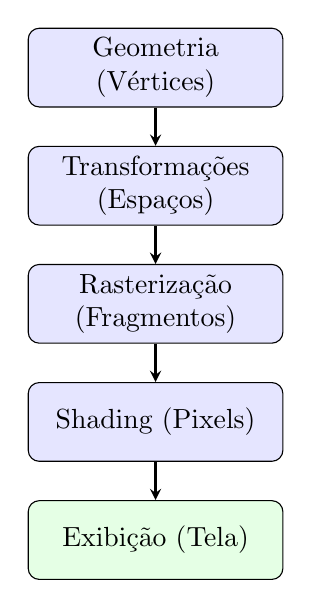
\begin{tikzpicture}[
    node distance=1.5cm,
    block/.style={rectangle, draw, fill=blue!10, text width=3cm, text centered, rounded corners, minimum height=1cm},
    arrow/.style={thick,->,>=stealth}
]
    \node (geo) [block] {Geometria (Vértices)};
    \node (trans) [block, below of=geo] {Transformações (Espaços)};
    \node (rast) [block, below of=trans] {Rasterização (Fragmentos)};
    \node (shading) [block, below of=rast] {Shading (Pixels)};
    \node (display) [block, below of=shading, fill=green!10] {Exibição (Tela)};

    \draw [arrow] (geo) -- (trans);
    \draw [arrow] (trans) -- (rast);
    \draw [arrow] (rast) -- (shading);
    \draw [arrow] (shading) -- (display);
\end{tikzpicture}
\end{center}

De forma detalhada, o processo segue estas etapas fundamentais descritas por \textcite{akenine2018realtime}:
\begin{enumerate}
    \item \textbf{Processamento de Vértices:} Aplicação de matrizes de transformação para posicionar objetos no mundo e projetá-los para a câmera.
    \item \textbf{Montagem de Primitivas:} Agrupamento de vértices em triângulos ou linhas.
    \item \textbf{Rasterização:} Conversão da geometria contínua em fragmentos discretos. É aqui que determinamos quais pixels do monitor são cobertos por cada triângulo.
    \item \textbf{Processamento de Fragmentos:} Cálculo da cor final, aplicação de texturas e iluminação.
    \item \textbf{Operações de Per-Sample:} Testes de profundidade (z-buffer), stencil e mistura de cores (blending).
\end{enumerate}

\section{O Que Você Vai Aprender}

Este volume foca no "como" e no "porquê". Não ensinaremos a usar uma ferramenta específica como Blender ou Unity, mas sim a matemática e os algoritmos que estas ferramentas utilizam. O objetivo é que, ao final da leitura, você consiga implementar seu próprio motor de renderização ou escrever \textit{shaders} complexos com total domínio técnico. Exploraremos desde a geometria básica até as sutilezas da luz e sombra, preparando-o para os desafios reais do desenvolvimento de software gráfico de alto desempenho.

\begin{aviso}
    Este volume não cobre animação de personagens, simulação física avançada ou técnicas de inteligência artificial aplicadas a gráficos. Esses temas serão abordados em volumes futuros.
\end{aviso}

\section{Pré-requisitos}

Para aproveitar este conteúdo, é essencial ter uma base sólida em:
\begin{itemize}
    \item \textbf{Álgebra Linear:} Vetores, matrizes, produtos escalares e vetoriais, e transformações espaciais são a linguagem da computação gráfica.
    \item \textbf{Cálculo:} Entender derivadas e integrais é vital para compreender a equação de renderização e modelos de iluminação avançados.
    \item \textbf{Programação:} Familiaridade com linguagens de baixo nível ou C-like (C++, C\#, Java ou GLSL) ajudará na compreensão dos algoritmos e na implementação prática dos projetos.
\end{itemize}

\begin{dica}
    Não se sinta intimidado pela matemática. Como afirma \textcite{shirley2021fundamentals}, a computação gráfica é visual. Sempre que encontrar uma fórmula difícil, tente desenhá-la. A intuição geométrica é sua melhor aliada. A prática constante de converter fórmulas em código é o que solidifica o conhecimento.
\end{dica}

\section*{Exercícios}

\begin{exercicio}{Fundamentos Históricos}
    Pesquise sobre o sistema \textit{Sketchpad} de Ivan Sutherland. Quais conceitos introduzidos por ele ainda são usados na computação gráfica moderna? Como a interação direta mudou o paradigma da computação na época?
\end{exercicio}

\begin{exercicio}{Tempo Real vs Offline}
    Explique a diferença fundamental entre renderização em tempo real (\textit{Real-Time Rendering}) e renderização \textit{Offline}. Cite exemplos de hardware e software típicos para cada uma e discuta o compromisso entre qualidade visual e velocidade.
\end{exercicio}

\begin{exercicio}{Importância da Matemática}
    Por que a computação gráfica depende tanto da Álgebra Linear? Dê um exemplo prático de como uma rotação de um objeto 3D é representada matematicamente e como isso é processado pela GPU.
\end{exercicio}

\begin{exercicio}{A Equação de Renderização}
    Como o trabalho de \textcite{kajiya1986rendering} mudou a forma como pensamos sobre a luz em ambientes digitais? Explique o conceito de iluminamento global que esta equação tenta formalizar.
\end{exercicio}

\begin{exercicio}{Aplicações Diversas}
    Cite três áreas fora do entretenimento onde a computação gráfica é essencial e descreva o benefício gerado. Como a visualização científica pode auxiliar na descoberta de novos medicamentos?
\end{exercicio}

\begin{exercicio}{Unidades Radiométricas}
    Diferencie Fluxo Radiante, Irradiância e Radiância. Se uma fonte de luz emite 100 Watts uniformemente em todas as direções, qual será a irradiância em uma esfera de raio 2 metros centrada na fonte?
\end{exercicio}

\begin{exercicio}{Arquitetura de Hardware}
    Explique os conceitos de SIMD e SIMT. Por que um processador com centenas de núcleos simples (GPU) é mais eficiente para renderização do que um processador com poucos núcleos complexos (CPU)?
\end{exercicio}

\begin{exercicio}{O Papel da BRDF}
    Na equação de renderização, qual é a função do termo $f_r$? Como você descreveria a BRDF de um espelho perfeito comparada a uma superfície de gesso fosco?
\end{exercicio}
